\section{灵敏度分析}\label{sec:sens}

达标时刻 $t^*$ 是本文的核心输出，其可信度取决于对关键假设的稳健性。本节逐项扰动
环境外推方式、蒸发潜热、是否计入收缩、界面平均方式，考察 $t^*$ 的相对变化，
总览见图~\ref{fig:sensitivity_tornado}。

\begin{figure}[H]
  \centering
  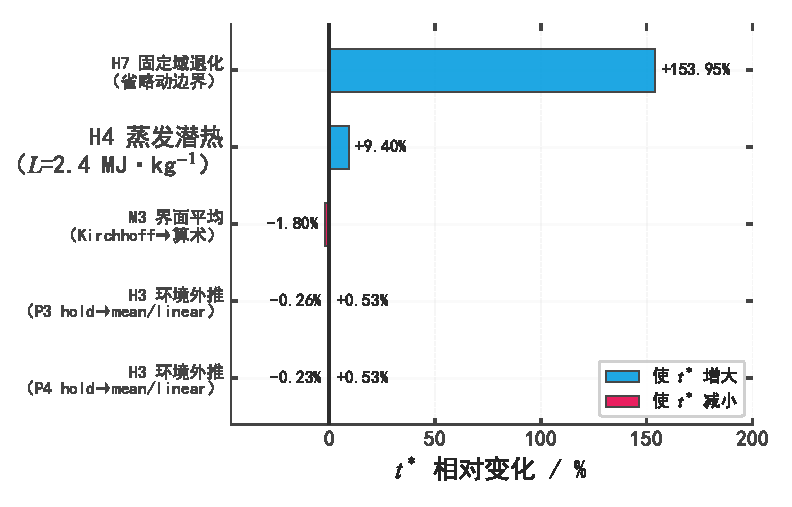
\includegraphics[width=0.9\textwidth,height=0.8\textheight,keepaspectratio]{../figures/fig_sensitivity_tornado.pdf}
  \caption{各假设扰动对达标时刻 $t^*$ 的相对影响（龙卷风图）}
  \label{fig:sensitivity_tornado}
\end{figure}

图~\ref{fig:sensitivity_tornado} 按影响幅度排序，各扰动的具体数值见表~\ref{tab:sensitivity}。

\begin{table}[H]
  \centering
  \caption{关键假设扰动对达标时刻的影响}
  \label{tab:sensitivity}
  \small
  \begin{tabular}{lrrr}
    \toprule
    扰动情景 & 基准 $t^*$ / h & 扰动 $t^*$ / h & 相对变化 \\
    \midrule
    问题3 环境保持$\to$区间均值   & 57.262 & 57.567  & $+0.53\%$ \\
    问题3 环境保持$\to$线性外推   & 57.262 & 57.115  & $-0.26\%$ \\
    问题4 环境保持$\to$区间均值   & 50.898 & 51.166  & $+0.53\%$ \\
    问题4 环境保持$\to$线性外推   & 50.898 & 50.782  & $-0.23\%$ \\
    计入蒸发潜热 $L=2.4$ MJ$\cdot$kg$^{-1}$ & 57.262 & 62.646 & $+9.40\%$ \\
    问题4 忽略收缩（退化为固定域） & 50.898 & 129.253 & $+153.95\%$ \\
    界面平均 Kirchhoff$\to$算术    & 57.262 & 56.230  & $-1.80\%$ \\
    界面平均 Kirchhoff$\to$调和    & 57.262 & 557.761 & $+874.05\%$ \\
    \bottomrule
  \end{tabular}

  \vspace{2pt}
  \parbox{0.94\linewidth}{\footnotesize
  注：附件1 仅覆盖前 $4\,\mathrm{h}$，对其后的环境外推（保持末值/区间均值/线性外推）影响
  不足 $0.6\%$，说明 $t^*$ 对外推方式稳健。蒸发潜热单向延长干燥期，因题面未给 $L$，
  基准不含潜热汇并作为下界报告。忽略收缩使 $t^*$ 虚高约 $1.5$ 倍，证实动边界为问题4 的
  必要机制。调和平均在 $D$ 跨三个量级时被最小值锁死，产生 $557.76\,\mathrm{h}$ 的非物理结果，
  故界面扩散系数采用 Kirchhoff 积分平均。}
\end{table}

由图~\ref{fig:sensitivity_tornado} 与表~\ref{tab:sensitivity} 可得三点结论：其一，\textbf{环境外推
方式影响极小}（$<0.6\%$），说明附件1 数据虽只覆盖前段，但因干燥后期由内部扩散控制、对边界
细节不敏感，$t^*$ 依旧稳健；其二，\textbf{是否计入收缩是最主要的建模选择}，忽略收缩会使 $t^*$
虚高 $1.5$ 倍以上，与图~\ref{fig:orthogonal_waterfall} 的正交分解相互印证；其三，界面平均方式中
调和平均产生非物理的 $557.76\,\mathrm{h}$，而 Kirchhoff 与算术平均相差仅 $1.80\%$，佐证
\ref{sub:kirchhoff} 节采用 Kirchhoff 积分平均的必要性与合理性。潜热项作为下界修正，提示
若实际工况散热更强，达标时间会相应延长约 $9\%$。
